\documentclass{article}
\usepackage{ctex}
\usepackage{graphicx}
\usepackage{amsmath}
\usepackage{indentfirst}
\usepackage{titlesec}
\usepackage{setspace}
\usepackage{subfigure}
\usepackage{caption}
\usepackage{float}
\usepackage{booktabs}
\usepackage{geometry}
\usepackage{multirow}
\geometry{left=1.2cm,right=1.2cm,top=2cm,bottom=2cm}
\title{\songti \zihao{2}\bfseries 磁光效应实验报告}
\titleformat*{\section}{\songti\zihao{4}\bfseries}
\titleformat*{\subsection}{\songti\zihao{5}\bfseries}
\renewcommand\thesection{\arabic{section}}
\author{王启骅 PB20020580}
\begin{document}
	\maketitle
\section{实验数据与处理}
注:本次实验由于激光光源功率过大(已使用最小光阑),这里采用$ \delta=0.5^{\circ} $

\begin{table}[!h]
	\centering
	\captionsetup{font={small},labelfont=bf}
	\caption{\heiti\zihao{-5}下降过程电压-电流关系}
	\begin{tabular}{|c|c|c|c|c|c|c|c|c|c|c|c|c|c|c|}
		
		\hline
		I/A&3.0&2.8&2.6&2.4&2.2&2.0&1.8&1.6&1.4&1.2&1.0\\
		\hline
		U/V&0.417&0.427&0.436&0.448&0.465&0.478&0.494&0.506&0.520&0.534&0.549\\
		\hline
		I/A&0.8&0.6&0.4&0.2&0.0&-0.2&-0.4&-0.6&-0.8&-1.0&-1.2\\
		\hline
		U/V&0.561&0.575&0.587&0.600&0.614&0.625&0.629&0.652&0.666&0.683&0.696\\
		\hline
		I/A&-1.4&-1.6&-1.8&-2.0&-2.2&-2.4&-2.6&-2.8&-3.0&&\\
		\hline
		U/V&0.713&0.727&0.744&0.765&0.784&0.812&0.838&0.865&0.884&&\\
		\hline
	\end{tabular}
\end{table}
	\begin{table}[!h]
		\centering
		\captionsetup{font={small},labelfont=bf}
		\caption{\heiti\zihao{-5}上升过程电压-电流关系}
		\begin{tabular}{|c|c|c|c|c|c|c|c|c|c|c|c|c|c|c|}
			
			\hline
			I/A&-3.0&-2.8&-2.6&-2.4&-2.2&-2.0&-1.8&-1.6&-1.4&-1.2&-1.0\\
			\hline
			U/V&0.884&0.873&0.865&0.840&0.819&0.798&0.777&0.754&0.736&0.719&0.704\\
			\hline
			I/A&-0.8&-0.6&-0.4&-0.2&0.0&0.2&0.4&0.6&0.8&1.0&1.2\\
			\hline
			U/V&0.688&0.671&0.658&0.643&0.632&0.618&0.606&0.595&0.578&0.571&0.556\\
			\hline
			I/A&1.4&1.6&1.8&2.0&2.2&2.4&2.6&2.8&3.0&&\\
			\hline
			U/V&0.544&0.529&0.511&0.501&0.482&0.468&0.447&0.429&0.418&&\\
			\hline
		\end{tabular}
	\end{table}

\begin{table}[!h]
	\centering
	\captionsetup{font={small},labelfont=bf}
	\caption{\heiti\zihao{-5}磁场-电流关系}
	\begin{tabular}{|c|c|c|c|c|c|c|c|c|c|c|c|c|c|c|}
		
		\hline
		-I/A&3.0&2.8&2.6&2.4&2.2&2.0&1.8&1.6&1.4&1.2&1.0\\
		\hline
		B/mT&100&94&88&82&75&69&62&56&49&42&35\\
		\hline
		-I/A&0.8&0.6&0.4&0.2&0.0&-0.2&-0.4&-0.6&-0.8&-1.0&-1.2\\
		\hline
		B/mT&29&22&15&9&2&-5&-11&-18&-25&-31&-38\\
		\hline
		-I/A&-1.4&-1.6&-1.8&-2.0&-2.2&-2.4&-2.6&-2.8&-3.0&&\\
		\hline
		B/mT&-45&-52&-58&-65&-71&-78&-84&-90&-96&&\\
		\hline
	\end{tabular}
\end{table}
	\section{数据处理}
	\begin{figure}[!h]
		
		\centering
		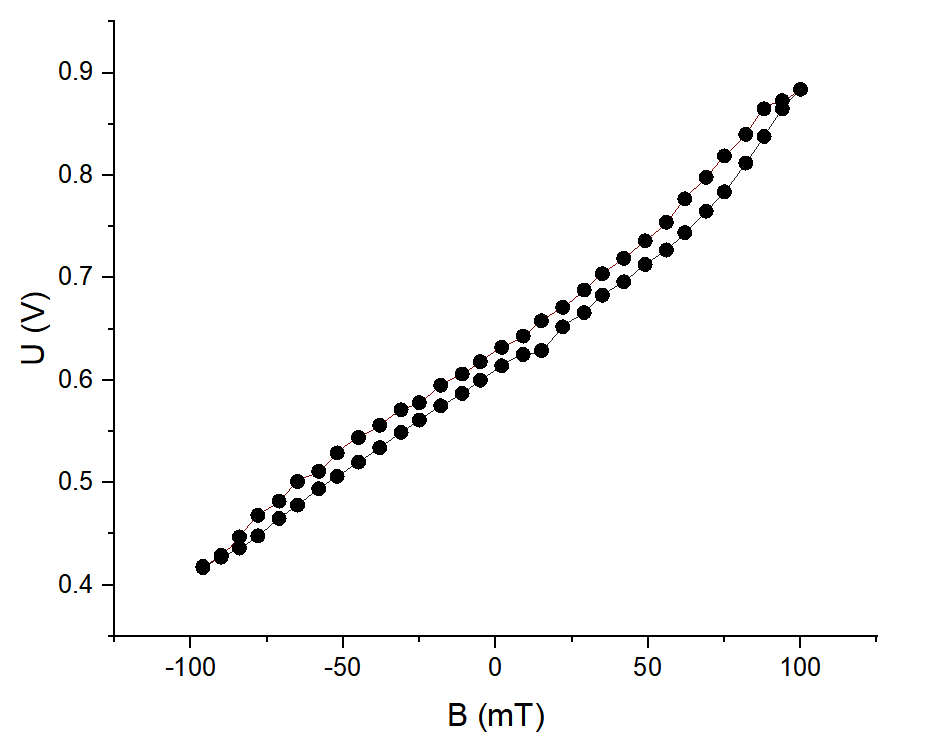
\includegraphics[scale=0.7]{磁滞回线}
		\captionsetup{font={small},labelfont=bf}
		\caption{\heiti\zihao{-5}磁滞回线结果}
		
	\end{figure}


\begin{equation}
	\theta_k^+=\frac{0.5^{\circ}}{2}\frac{I-I_0}{I_0}=\frac{0.5^{\circ}}{2}\frac{0.884-0.614}{0.614}=0.110^{\circ}
\end{equation}

\begin{equation}
	\theta_k^-=\frac{0.5^{\circ}}{2}\frac{I-I_0}{I_0}=\frac{0.5^{\circ}}{2}\frac{0.417-0.614}{0.614}=-0.080^{\circ}
\end{equation}
极向克尔旋转角
\begin{equation}
	\theta_k=\frac{1}{2}(\theta_k^+-\theta_k^-)=0.095^{\circ}
\end{equation}

\section{思考题}
1.磁光克尔效应测量实验中, $ \delta $的大小该如何选取?如果过大或过小分别会对测量有什么样的影响?


按照原理近似的要求,需要$ \delta<<1(rad) $,这样才可以对$ \sin\delta\sim\delta,\cos\delta\sim1-\delta^2 $近似成立。同时$ \theta_k<<\delta $,才可以使近似$ I\simeq I_0(1+2\frac{\theta_k}{\delta}) $成立,因此需要适中选取。过大会导致$ \sin\delta<\delta $,计算结果偏大。过小时舍去$ \theta_k^2 $项不合理,也会导致结果偏大。


2.克尔效应测量实验中,加上一定的外加磁场后,反射光束是否还是线偏振光?如何通过我们的实验设备来判断?


是。可以转动检偏器偏振片,看到可以完全消光则仍是线偏振。


3.实验中如何判断克尔转角和法拉第旋转角的旋转方向?写出具体的判断过程。


加磁场前先调节为消光状态,加磁场后,有一定的转角,会导致有光信号,向两边细调检偏器,在某一方向会重新消光,则该旋转方向为转角的方向。


4.法拉第效应测量实验中,起偏格兰棱镜的偏振方向是否需要精细调节,为什么?


不需要,由于垂直入射,整个实验过程与起偏镜的绝对角度无关,实验中只与起偏和检偏的相对夹角有关,则只精细调节检偏镜即可。


\end{document}